\documentclass[11pt, aspectratio=169]{beamer}
\usefonttheme[onlymath]{serif}

\setbeamersize{text margin left=1.5em}
\setbeamersize{text margin right=1.5em}

\setbeamertemplate{frametitle}{%
  \vskip1ex
  \usebeamerfont{frametitle}%
  \insertframetitle\par
  \vskip1ex
  \hrule
}

\setbeamertemplate{blocks}[rounded][shadow=true]

% Add numbered captions for figures/tables in beamer
\setbeamertemplate{caption}[numbered]

\setbeamertemplate{itemize item}{\usebeamerfont{itemize item}\textbullet}
\setbeamertemplate{itemize subitem}{\usebeamerfont{itemize subitem}\textbullet}
\setbeamertemplate{itemize subsubitem}{\usebeamerfont{itemize subsubitem}\textbullet}

\makeatletter
\geometry{%
  papersize={\fpeval{\beamer@paperwidth*1.5}pt,\fpeval{\beamer@paperheight*1.5}pt},
  hmargin=\fpeval{0.5 * 1.0}cm,% 1cm
  vmargin=0cm,%
  head=\fpeval{0.5*1.5}cm,% 0.5cm
  headsep=0pt,%
  foot=\fpeval{0.5*1.5}cm% 0.5cm
}
\makeatother

\usepackage{booktabs}
\usepackage{graphicx}
\usepackage[dvipsnames]{xcolor} % <-- removed obsolete `usenames` option
\usepackage{amsmath}
\usepackage{amssymb}
\usepackage{mathtools}
\usepackage{subcaption}

\usepackage[
  backend=bibtex,
  style=authoryear,   % or numeric
  citestyle=authoryear
]{biblatex}
\addbibresource{../../references.bib}

% Your custom commands (kept as is)
\newcommand{\mrm}[1]{\mathrm{#1}}
\newcommand{\mbb}[1]{\mathbb{#1}}
\newcommand{\mb}[1]{\mathbf{#1}}
\newcommand{\mc}[1]{\mathcal{#1}}
\newcommand{\tb}[1]{\textbf{#1}}
\newcommand{\Unif}{\operatorname{Unif}}

\DeclareMathOperator{\diverg}{div}

% \DeclareMathOperator{\div}{\operatorname{div}}

\title{Flow Matching}
\author{Gwanwoo Choi}
\institute{MLIC}
\date{} % To use the current date

\begin{document}

\begin{frame}
    \titlepage
\end{frame}

\begin{frame}{Flow Matching Concept}
  \begin{block}{Problem Definition}
    \begin{columns}[t]
      \begin{column}{0.45\textwidth}
        \begin{figure}
      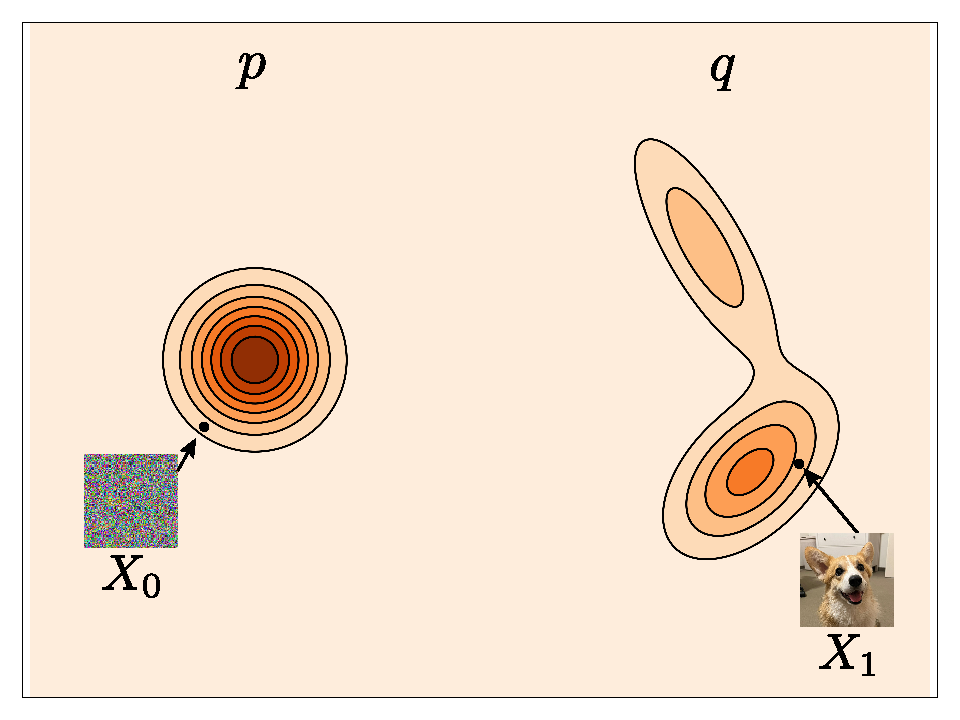
\includegraphics[width=0.6\textwidth]{assets/data.pdf}
      \caption{Data Distribution}
      \end{figure}

      \end{column}
      \begin{column}{0.50\textwidth}
        \begin{itemize}
          \item Let $q$ be the data distribution.
          \item Our objective is to \tb{learn a generative model} that can sample from $q$.
          \item Each data point is modeled as a random variable (r.v.) $X_1 \in \mathbb{R}^d$ with distribution $X_1 \sim q$.
          \item Modern generative models (e.g. VAE, Diffusion Models, Flow Matching) leverages an tractable distribution (e.g. Gaussian) to generate $X_1$.
          \item Let $q$ denote a known distribution chosen for modeling (e.g., a Gaussian), and let $X_0$ be a random variable with distribution $X_0 \sim p$.
        \end{itemize}
      \end{column}
    \end{columns}
  \end{block}
\end{frame}


\begin{frame}{Flow Matching Concept}

  \begin{block}{Differences between generative models}
    \begin{figure}
    \centering
    % Reduce spacing between the two images by using wider subfigures
    % and a small fixed horizontal gap. Keep images slightly inset with
    % includegraphics width < \subfigure width to avoid touching edges.
    \captionsetup[subfigure]{skip=0.5ex, labelfont=small, textfont=small}
    \begin{subfigure}[b]{0.30\textwidth}
      \centering
      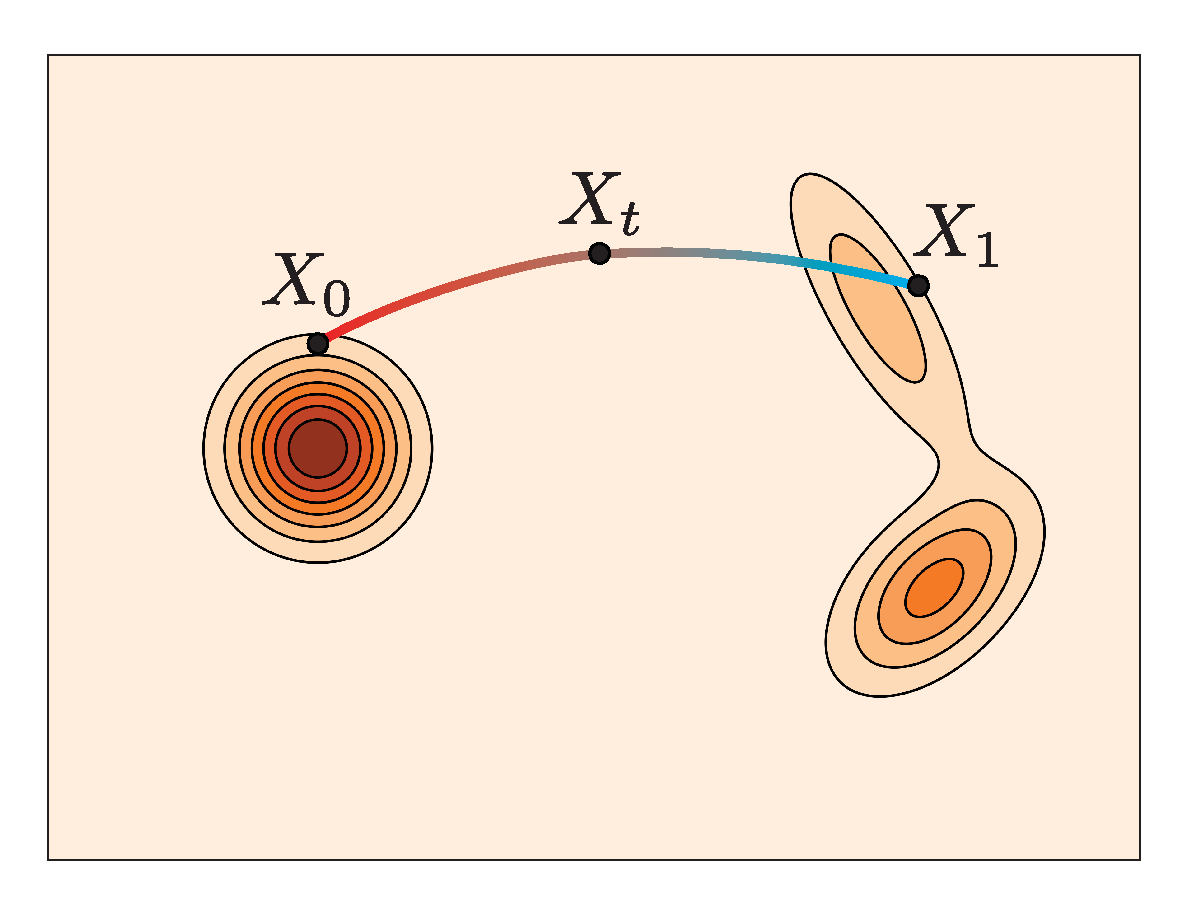
\includegraphics[width=0.9\textwidth]{assets/type_flow.pdf}
      \caption{Flow}
      \label{fig:types:flow}
    \end{subfigure}\hspace{0.02\textwidth}%
    \begin{subfigure}[b]{0.30\textwidth}
      \centering
      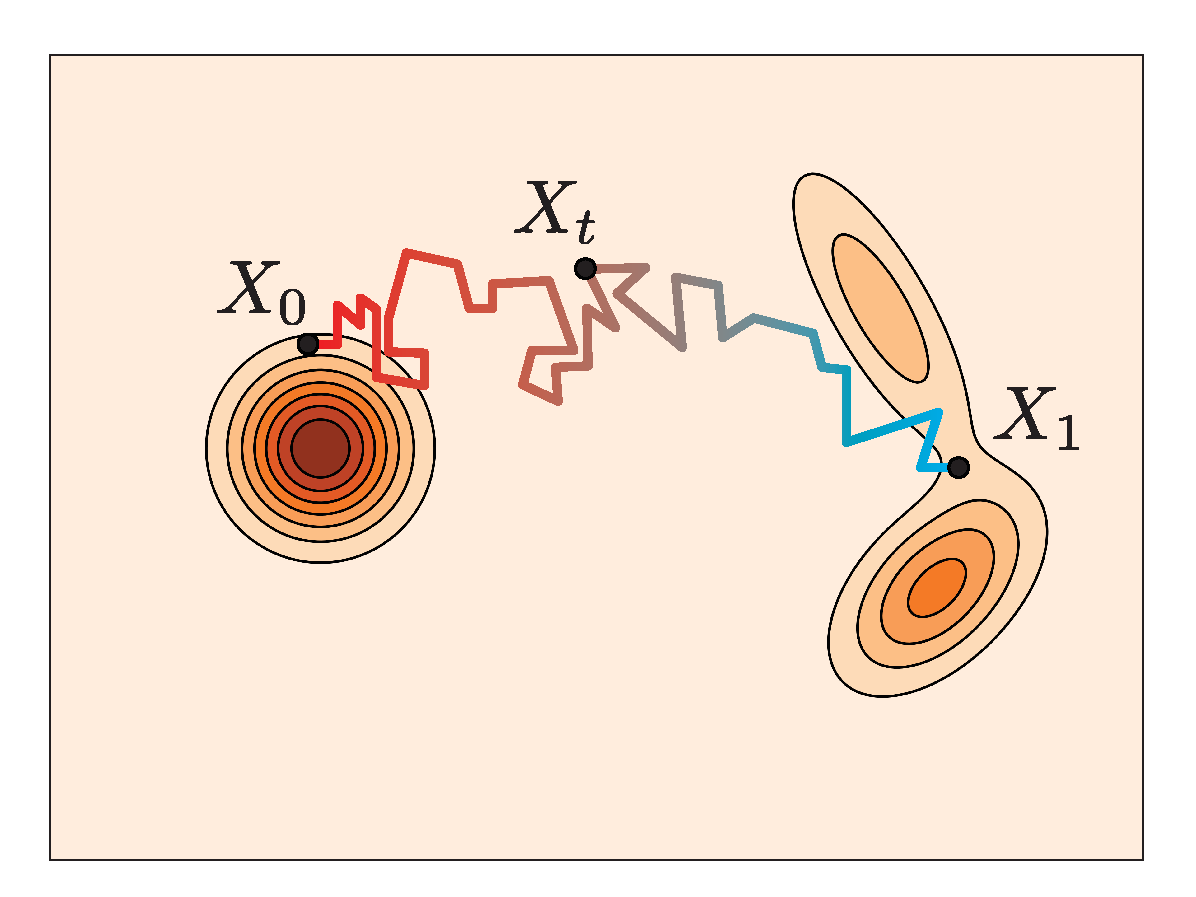
\includegraphics[width=0.9\textwidth]{assets/type_diffusion.pdf}
      \caption{Diffusion}
      \label{fig:types:diffusion}
    \end{subfigure}
    \caption{Difference between Flow Matching and Diffusion Models}
    \end{figure}

    \begin{itemize}
      \item Variational AutoEncoders (VAE): sample $x_0$ from a prior and use a deterministic decoder to produce $X_1$.
      \item Flow Matching: Construct a deterministic continuous flow (ODE-based) that transports $X_0$ to $X_1$.
      \item Diffusion models: generate $X_1$ by simulating a stochastic process (e.g. reverse-time SDE), so the mapping from $X_0$ to $X_1$ is stochastic.
    \end{itemize}
  \end{block}
\end{frame}

\begin{frame}{Flow Matching Concept}
  \begin{block}{Probability Path}
    \begin{columns}
      \begin{column}{0.45\textwidth}
        \begin{figure}
          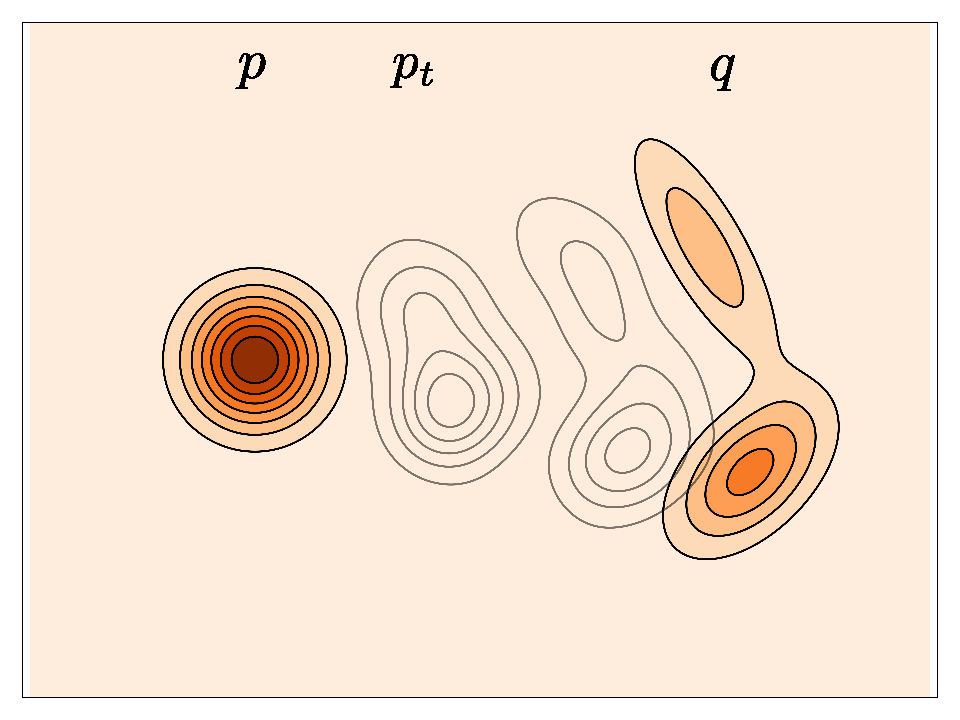
\includegraphics[width=0.6\textwidth]{assets/p_t.pdf}
          \caption{Probability Path}
        \end{figure}
      \end{column}
      \begin{column}{0.50\textwidth}
        \begin{itemize}
          \item Let define a \tb{probability path} $(p_t)_{0 \leq t \leq 1}$.
          \item The path $p_t$ is a \underline{continuous interpolation} between the known distribution $p$ and the data distribution $q$ such that $p_{0} = p$ and $p_{1} = q$.
          \item How can we find \underline{proper} $p_t$ for all $t \in [0,1]$ that matches boundary condition $p_0= p, p_1 = q$? ($\to$ Flow Matching.)
        \end{itemize}
      \end{column}
    \end{columns}
  \end{block}
\end{frame}

\begin{frame}{Basic Concept}
  \begin{block}{Flow \& Flow Model}
    \begin{itemize}
      \item A $C^r$ \tb{flow} is a \underline{time-dependent positional mapping} $\psi: [0,1] \times \mbb{R}^d \to \mbb{R}^d$ (here $C^r$ denotes functions whose derivatives up to order $r$ exist and are continuous).
      \item Let denote $\psi_t(x)$ as the \underline{position at time $t$ of a particle} that started at $x$ at time $t=0$ ($\psi: (t,x) \mapsto \psi_t(x)$).
      \item $\psi \in C^r$ and $\psi_t$ is a $C^r$ diffeomorphism.
      \item A \tb{Flow Model} is a \hyperlink{appendix:flow_model_markov}{\underline{continuous-time Markov process}} $(X_t)_{0 \leq t \leq 1}$ defined by applying a flow $\psi_t$ to the RV $X_0$.
      $$
        X_t = \psi_t(X_0),\ t \in [0,1], \text{ where } X_0 \sim p
      $$
      \item The \tb{goal of generative flow modeling} is to find a flow $\psi_t$ such that
      $$
        X_1 = \psi_1 (X_0) \sim q
      $$
    \end{itemize}
  \end{block}

  \begin{block}{Samples of Flow Model}
    \begin{figure}
      \centering
      \captionsetup[subfigure]{skip=0.5ex, labelfont=small, textfont=small}
      \begin{subfigure}[b]{0.23\textwidth}
        \centering
        \includegraphics[width=0.9\textwidth]{assets/flow_1_p.png}
        \caption{$X_0$}
      \end{subfigure}\hspace{0.02\textwidth}
      \begin{subfigure}[b]{0.23\textwidth}
        \centering
        \includegraphics[width=0.9\textwidth]{assets/flow_10_p.png}
        \caption{$X_t = \psi_t(X_0)$}
      \end{subfigure}\hspace{0.02\textwidth}
      \begin{subfigure}[b]{0.23\textwidth}
        \centering
        \includegraphics[width=0.9\textwidth]{assets/flow_16_p.png}
        \caption{$X_1 = \psi_1(X_0)$}
      \end{subfigure}
    \end{figure}
  \end{block}
\end{frame}

\begin{frame}{Basic Concept}
  \begin{block}{Equivalence between flows and velocity fields}
    \begin{itemize}
      \item Let denote $u_t(x)$ as the \underline{velocity} of a particle, which is positioned in $x$ at time $t=0$, at time $t$.
      \item A flow $\psi$ be defined in terms of a \tb{velocity field} $u: [0,1] \times \mbb{R}^d \to \mbb{R}^d$ via the following ODE:
      $$
      \begin{gathered}
        \frac{d}{dt} \psi_t(x) = u_t(\psi_t(x_0)) = u_t(x) \\
        \psi_0(x_0) = x_0
      \end{gathered}
      $$
    \end{itemize}
  \end{block}

  \begin{block}{Velocity fields}
    \begin{figure}
      \centering
      \captionsetup[subfigure]{skip=0.5ex, labelfont=small, textfont=small}
      \begin{subfigure}[b]{0.23\textwidth}
        \centering
        \includegraphics[width=0.9\textwidth]{assets/flow_1.png}
        \caption{$u_0$}
      \end{subfigure}\hspace{0.02\textwidth}
      \begin{subfigure}[b]{0.23\textwidth}
        \centering
        \includegraphics[width=0.9\textwidth]{assets/flow_10.png}
        \caption{$u_t$}
      \end{subfigure}\hspace{0.02\textwidth}
      \begin{subfigure}[b]{0.23\textwidth}
        \centering
        \includegraphics[width=0.9\textwidth]{assets/flow_16.png}
        \caption{$u_1$}
      \end{subfigure}
    \end{figure}
  \end{block}
\end{frame}

\begin{frame}{Basic Concept}
  \begin{block}{Push-forward (Change of variables)}
    \begin{itemize}
      \item \tb{Push-forward} describes how a probability \underline{distribution transforms under a mapping}.
      \item Given a RV $X \sim p_X$ with density $p_X$, let us consider a RV $Y = f(X)$, where $f: \mbb{R}^d \to \mbb{R}^d$ is a $C^1$ diffeomorphism and let $g = f^{-1}$ be its inverse mapping.
      \item The probability density function(PDF) of $Y$ is called the \tb{push-forward} of $p_X$ and denoted by $$[f_{\#}p_X](y) \triangleq p_X(f^{-1}(y))\lvert \det \partial_y \phi(y)\rvert= p_Y(y), \quad  \text{ where }[\partial_y g(y)]_{i,j} = \frac{\partial g^i}{\partial y^j}, i,j \in \{1,2,\dots, d\}$$
    \end{itemize}
  \end{block}

  \begin{block}{Probability Paths}
    \begin{columns}
      \begin{column}{0.3\textwidth}
        \begin{figure}
          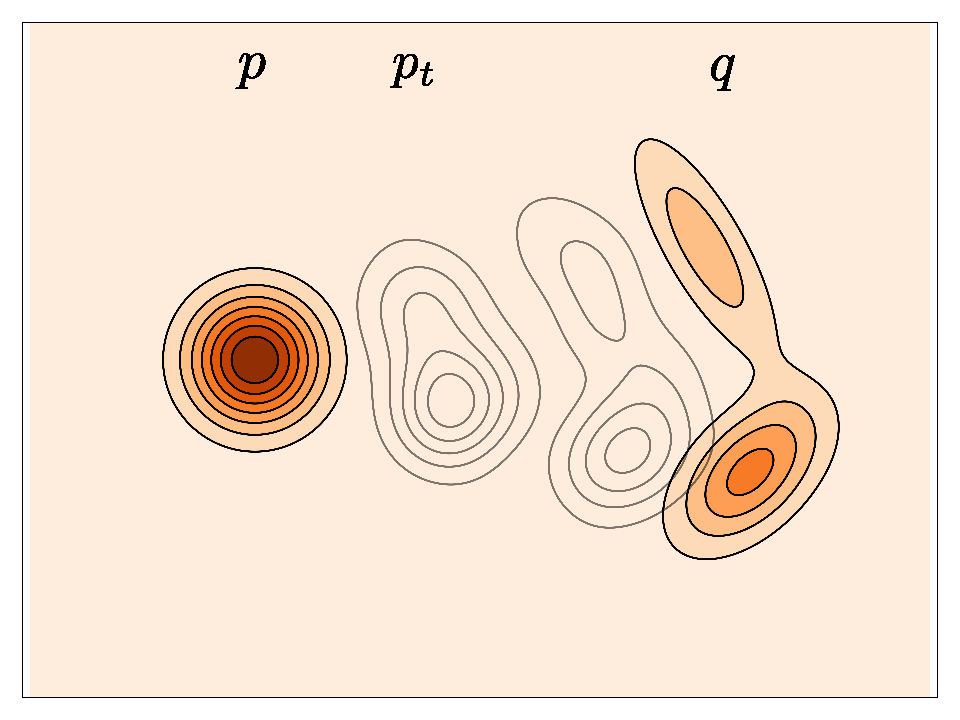
\includegraphics[width=0.9\textwidth]{assets/p_t.pdf}
        \end{figure}
      \end{column}
      \begin{column}{0.65\textwidth}
        \begin{itemize}
          \item We call a time-dependent probability $(p_t)_{0 \leq t \leq 1}$ a \tb{probability path}.
          \item For each time $t\in [0,1]$, these marginal PDFs are obtained via the push-forward formula
          $$
            p_t(x) = [\psi_{t \#} p](x)
          $$
          \item We call that $u_t$ \tb{generates} $p_t$ if $X_t = \psi_t(X_0) \sim p_t$ for all $t \in [0,1)$.
          \item The condition that $u_t$ can be generate $p_t$ is described in \hyperlink{appendix:continuity_equation_and_mass_conservation}{Appendix}.
        \end{itemize}
      \end{column}
    \end{columns}
  \end{block}
\end{frame}

\begin{frame}{Flow Matching}
  \begin{block}{Flow Matching Problem}
    \begin{itemize}
      \item In Flow Matching, we define a learnable velocity field $u_t^\theta$.
      \item \tb{Flow Matching Problem}: \underline{Find $u^\theta_t$ generating $p_t$, with satisfy boundary conditions $p_0=p$ and $p_1=q$}.
    \end{itemize}
    \begin{figure}
      \centering
      \captionsetup[subfigure]{skip=0.5ex, labelfont=small, textfont=small}
      \begin{subfigure}[b]{0.24\textwidth}
        \centering
        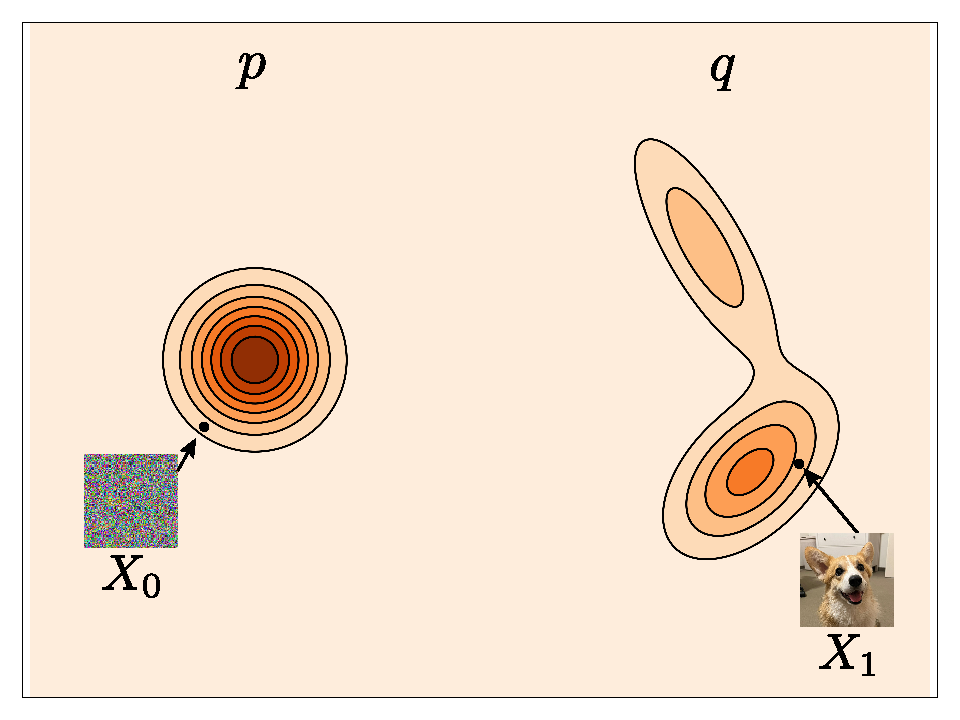
\includegraphics[width=0.9\textwidth]{assets/data.pdf}
        \caption{Data}
      \end{subfigure}
      \begin{subfigure}[b]{0.24\textwidth}
        \centering
        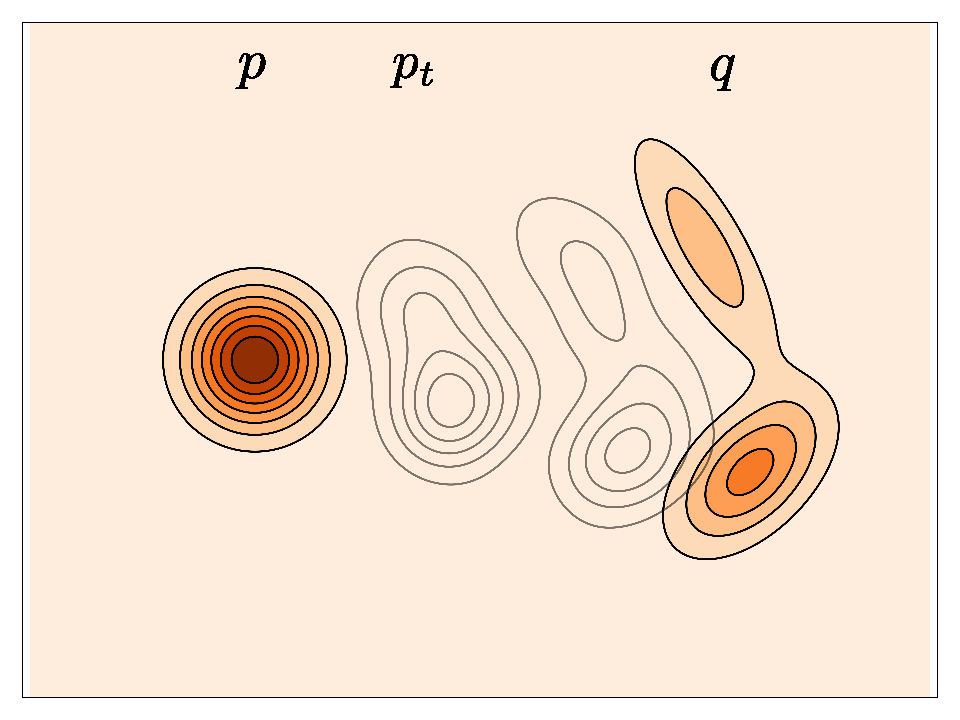
\includegraphics[width=0.9\textwidth]{assets/p_t.pdf}
        \caption{Path Design}
      \end{subfigure}
      \begin{subfigure}[b]{0.24\textwidth}
          \centering
          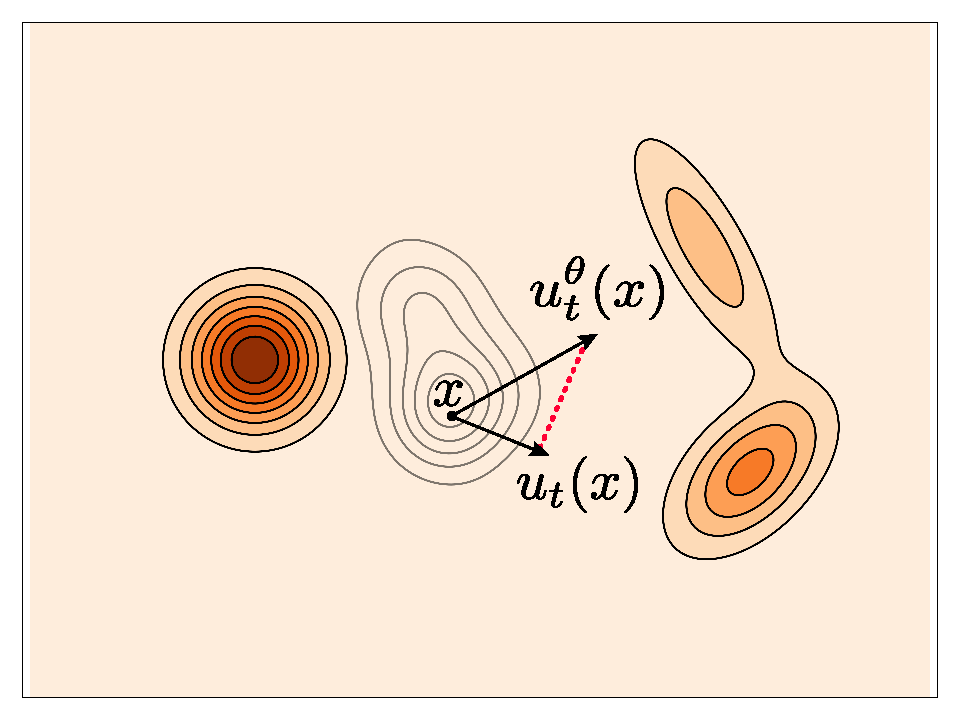
\includegraphics[width=0.9\textwidth]{assets/match_pt.pdf}
          \caption{Training}
      \end{subfigure}
          \begin{subfigure}[b]{0.24\textwidth}
        \centering
        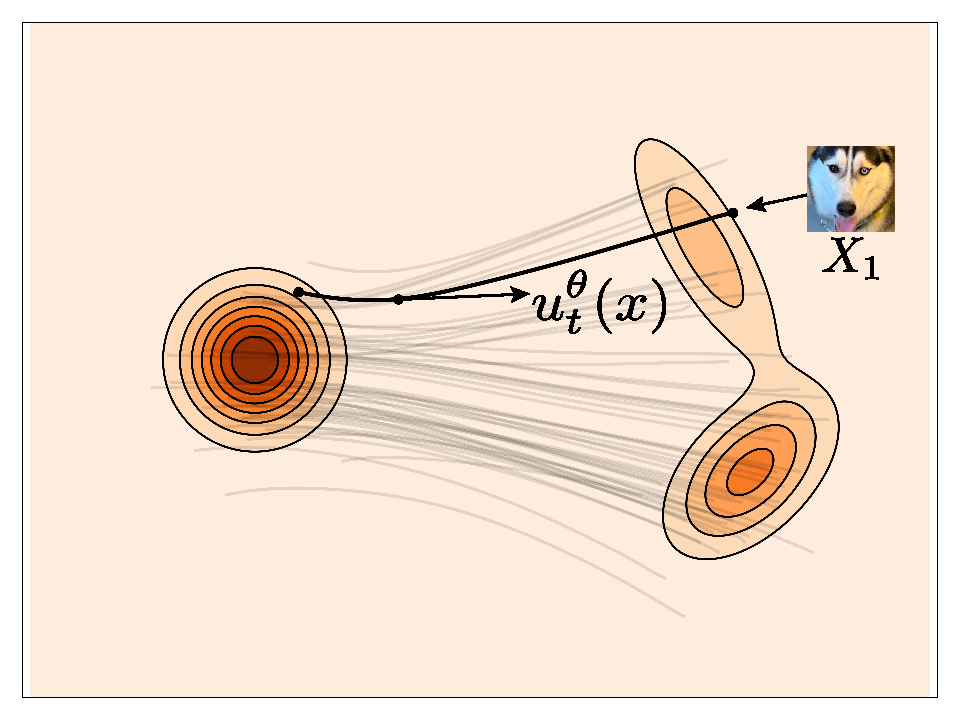
\includegraphics[width=0.9\textwidth]{assets/fm_recepie_4.pdf}
        \caption{Sampling}
      \end{subfigure}
    \end{figure}
    \begin{itemize}
      \item (a) identifies a known source distribution $p$ and an unknown data target distribution $q$
      \item (b) predescribe a probability path $p_t$ interpolating from $p_0 =p$ to $p_1 = q$
      \item (c) learns a velocity field $u^\theta_t$ implemented in terms of a neural network and generating the path $p_t$
      \item (d) samples from the learned model by solving an ODE with $u_t^\theta$
    \end{itemize}
  \end{block}
\end{frame}

\begin{frame}{Flow Matching}
  \begin{block}{Building probability paths}
    \begin{columns}
      \begin{column}{0.4\textwidth}
        \begin{figure}
          \centering
          \captionsetup[subfigure]{skip=0.5ex, labelfont=small, textfont=small}
          \begin{subfigure}[b]{0.48\textwidth}
            \centering
            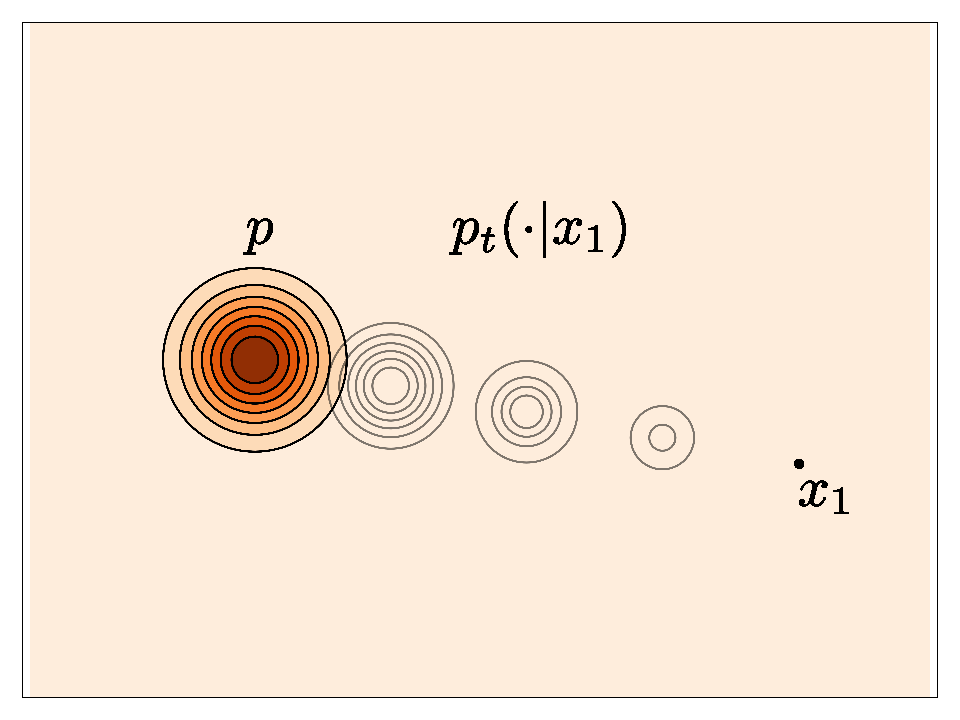
\includegraphics[width=0.9\textwidth]{assets/p_cond.pdf}
            \caption{Conditional probability path $p_{t|1}(x|x_1)$}
          \end{subfigure}\hfill
          \begin{subfigure}[b]{0.48\textwidth}
            \centering
            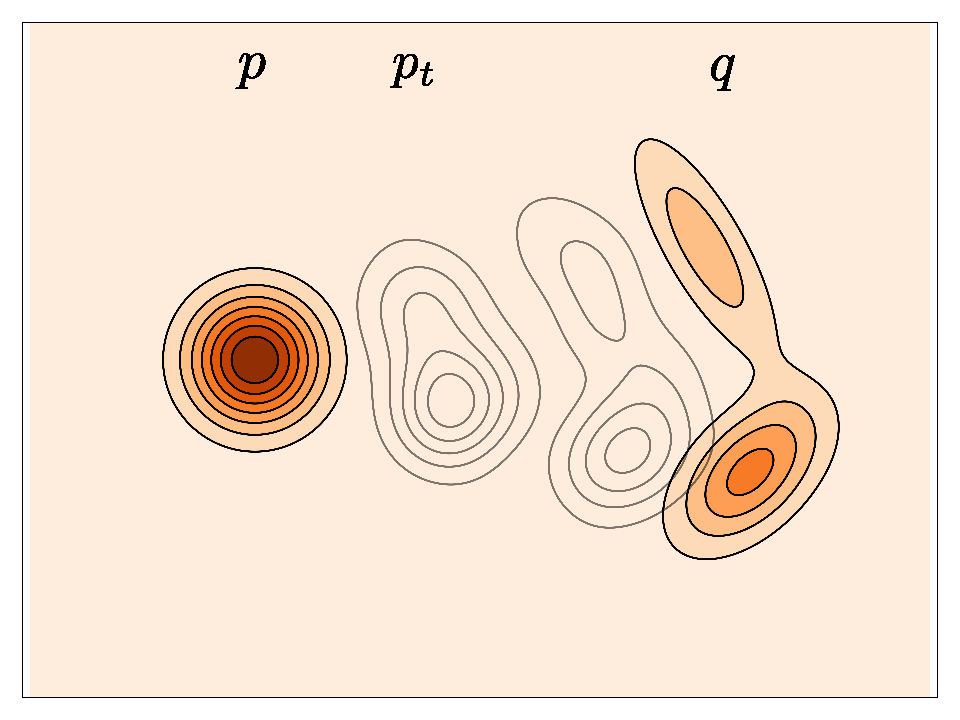
\includegraphics[width=0.9\textwidth]{assets/p_t.pdf}
            \caption{(Marginal) probability path $p_t(x)$}
          \end{subfigure}
        \end{figure}
      \end{column}
      \begin{column}{0.55\textwidth}
        \begin{itemize}
          \item Flow Matching drastically simplifies the problem of designing a probability path $p_t$ by adopting a \textit{conditional} strategy.
          \item Consider conditioning the design of $p_t$ on a single target example $X_1 = x_1$, yielding the \tb{conditional probability path} $p_{t|1}(x|x_1)$
          \item Then we may construct the overall, \tb{marginal probability path} $p_t$ by aggregating such conditional probability paths $p_{t|1}$
          $$
            p_t(x) =\int p_{t|1}(x|x_1)q(x_1)dx_1
          $$
          \item \underline{By setting as following, we can meet the boundary conditions} $p_0 = p$ and $p_1 = q$, where $\pi_{0|1}(x_0|x_1) = \pi_{0,1}(x_0, x_1)/q(x_1) = p(x_0) q(x_1)/q(x_1) = p(x_0)$ and $\delta_{x_1}$ is the delta meausre centered at $x_1$.
          $$
          \begin{gathered}
            p_{0|1}(x_0|x_1) = \pi_{0|1}(x_0|x_1) = \pi_{0,1}(x_0, x_1)/q(x_1) = p(x_0) \\ \quad p_{1|1}(x|x_1) = \delta_{x_1}(x)
          \end{gathered}
          $$
          \item For example, $p$ is a Gaussian distribution and $p_t$ is defined by linear interpolation between $p$ and $q$.
          $$
          \mc{N}(\cdot|t x_1, (1-t)^2 I) \to \delta_{x_1}(\cdot) \text{ as } t \to 1
          $$
        \end{itemize}
      \end{column}
    \end{columns}
  \end{block}
\end{frame}

\begin{frame}{Flow Matching}
  \begin{block}{Deriving generating velocity fields}
    \begin{columns}
      \begin{column}{0.4\textwidth}
        \begin{figure}
          \centering
          \captionsetup[subfigure]{skip=0.5ex, labelfont=small, textfont=small}
          \begin{subfigure}[b]{0.48\textwidth}
            \centering
            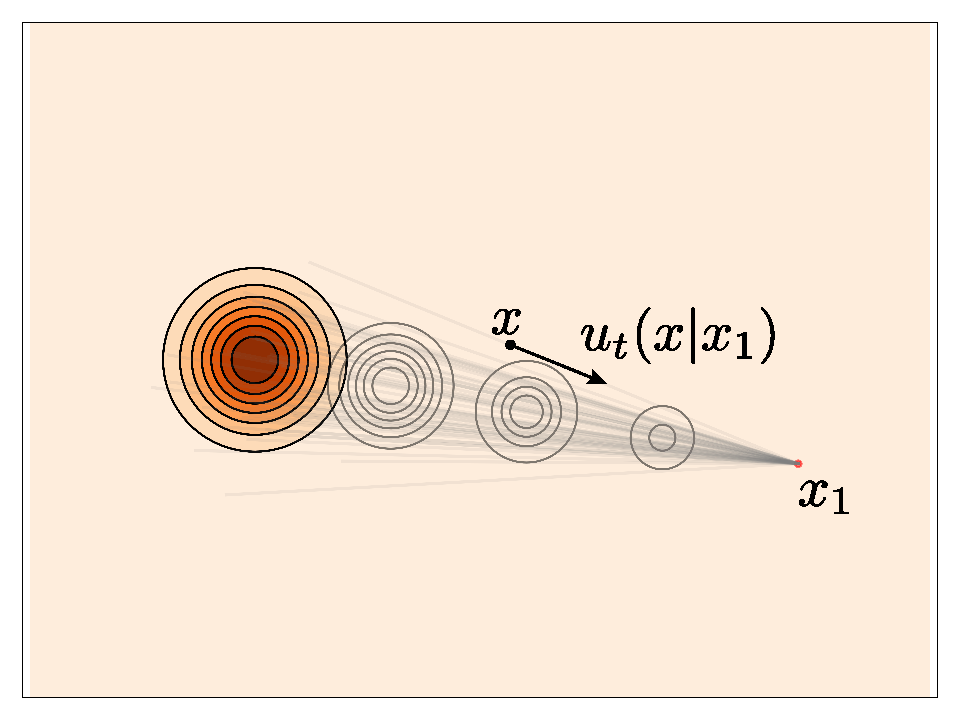
\includegraphics[width=0.9\textwidth]{assets/fm_recepie_2.pdf}
            \caption{Conditional velocity field $u_t(x|x_1)$}
          \end{subfigure}\hfill
          \begin{subfigure}[b]{0.48\textwidth}
            \centering
            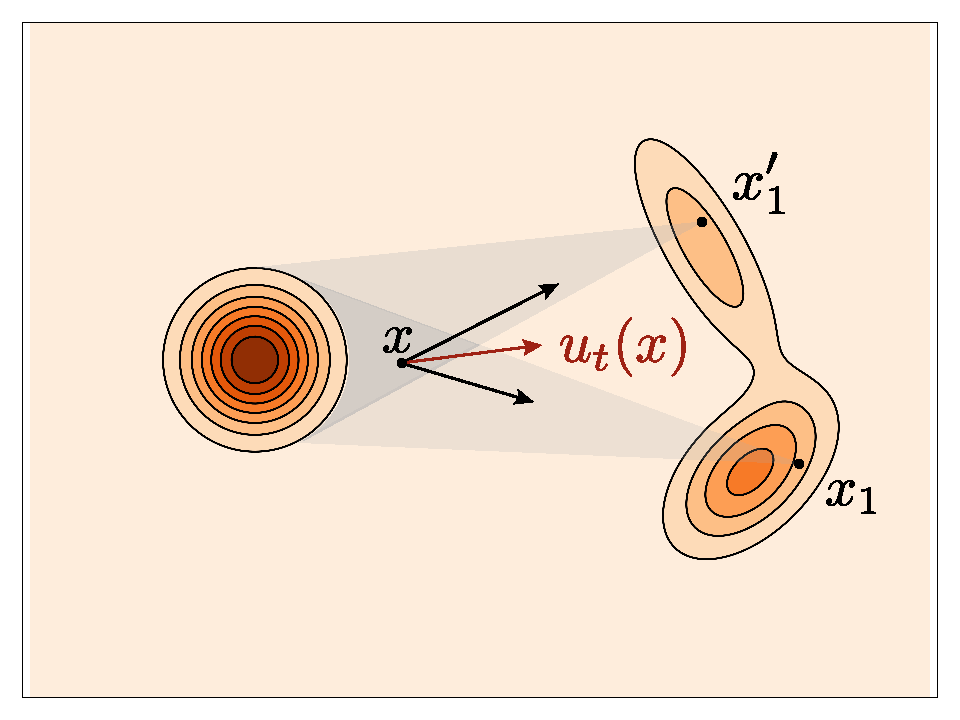
\includegraphics[width=0.9\textwidth]{assets/cond_E_u.pdf}
            \caption{(Marginal) Velocity field $u_t(x)$}
          \end{subfigure}
        \end{figure}
      \end{column}
      \begin{column}{0.55\textwidth}
        \begin{itemize}
          \item Let define $u_t(x|x_1)$ be the \tb{conditional velocity fields} that satisfying
          $$
            u_t(\cdot|x_1) \tb{ \text{generates} } p_{t|1}(\cdot|x_1)
          $$
          % \item For example, we can define $u_{t|1}(x|x_1) \triangleq \frac{x_1 - x}{1-t}$ and this $u_{t|1}$ generates $p_{t|1}$.
          \item The \tb{marginal velocity field} $u_t(x)$, which generates the marginal path $p_t(x)$, is given by averaging theconditional velocity fields $u_t(x|x_1)$ across target examples:
          $$
          \begin{aligned}
            u_t(x) &= \int u_t(x|x_1) p_{t|1}(x|x_1) dx_1 = \int u_t(x|x_1) \frac{p_{t|1}(x|x_1)q(x_1)}{p_t(x)} dx_1 \\&= \mbb{E}_{X_1 \sim q} [u_t (X_t|X_1) |X_t = x]
          \end{aligned}
          $$
          \item It is shonw that this \underline{marginal $u_t(x)$ velocity field generates the marginal probability path $p_t(x)$} if $u_t(\cdot|x_1)$ \tb{generates} $p_{t|1}(\cdot|x_1)$.
          \item For example, let $p_{t|1}(x|x_1) = \mc{N}(x|tx_1, (1-t)^2I)$. Then $u_{t|1}(x|x_1) =(x_1 - x)/(1-t)$ generates $p_{t|1}(x|x_1)$.
        \end{itemize}
      \end{column}
    \end{columns}
  \end{block}
\end{frame}

\begin{frame}{Flow Matching}
  \begin{block}{Flow Matching Loss}
    \begin{itemize}
      \item Let denote $D(u,v)$ as the \hyperlink{appendix:bregman_divergence}{bregman divergence}, which measures dissimilarity between two vectors $u$ and $v$ (e.g. $D(u,v) = \lVert u - v \rVert^2_2$).
      \item Let denote $\mc{L}_{\text{FM}}(\theta) = \mbb{E}_{\substack{t \sim \Unif[0,1] \\ X_t \sim p_t}}  D(u_t(X_t), u^\theta_t(X_t))$ the \tb{Flow Matching Loss} and $u_t^\theta$ be a learnable velocity field parameterized by $\theta$.
      \item Let denote $\mc{L}_{\text{CFM}}(\theta) = \mbb{E}_{\substack{t \sim \Unif[0,1] \\ X_1 \sim q \\ X_t \sim p_t}}  D(u_t(X_t|X_1), u^\theta_t(X_t))$ the \tb{Conditional Flow Matching Loss}.
      \item What we want to know is true velocity field $u_t$ that generates $p_t$.
      \item However, \underline{it is intractable to compute $u_t$ directly. Unlike $u_t$, the conditional velocity field $u_{t|1}$ is \tb{tractable}.}
      \item Fortunately, it is shown that
      $$
        \nabla_\theta \mc{L}_{\text{FM}}(\theta) = \nabla_\theta \mc{L}_{\text{CFM}}(\theta)
      $$
      \item So, we can optimize the learnable velocity field $u_t^\theta$ by minimizing the \tb{tractable} CFM loss.
    \end{itemize}
  \end{block}
\end{frame}

\begin{frame}{Flow Matching}
  \begin{block}{Problem formulation}
    So far, wehave reducedthe problem of training a flow model
    \begin{enumerate}
      \item Find conditional probability paths $p_{t|1}(x|x_1)$ yielding a marginal probability path $p_t(x)$ satisfying the boundary conditions.
      \item Find conditional velocity fields $u_t(x|x_1)$ generating the conditional probability path.
      \item Train using the CFM loss.
    \end{enumerate}
    We now discuss a concrete options on how to do step $1$. and $2$.
  \end{block}
\end{frame}

\begin{frame}{Flow Matching}
  \begin{block}{Conditional flows}
    \begin{columns}
      \begin{column}{0.3\textwidth}
        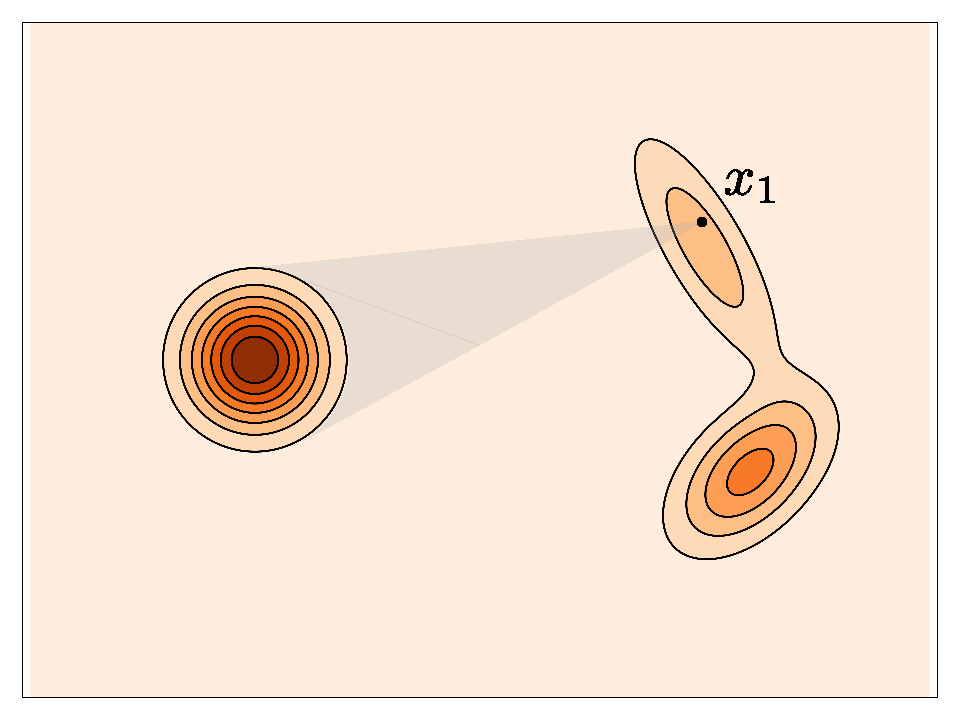
\includegraphics[width=0.95\textwidth]{assets/x1_cond.pdf}
      \end{column}
      \begin{column}{0.65\textwidth}
        \begin{itemize}
          \item Define the \tb{conditional flow model} $X_{t|1}$ by
          $$
            X_{t|1} = \psi_t(X_0 |x_1), \text{ where } X_0 \sim \pi_{0|1}(\cdot|x_1)
          $$
          where $\psi: [0,1) \times \mbb{R}^d \times \mbb{R}^d \to \mbb{R}^d$ is a \tb{conditional flow} that satisfies
          $$
            \psi_t(x_0|x_1)= \begin{cases}
              x_0 &t=0 \\ x_1 & t=1
            \end{cases}
          $$
          \item It is known that  there exists a unique smooth conditional velocity field, where $x = \psi_t(x_0|x_1)$
          $$
            u_t(x|x_1) = \frac{d}{dt} \psi_t (\psi^{-1}_t (x|x_1)|x_1) = \frac{d}{dt} \psi_t (x_0|x_1)
          $$
          \item By the Law of Unconscious Statistician, following holds
          $$
            u_t(x) =\frac{d}{dt} \psi_t (x_0|x_1) =\mbb{E}_{X_t \sim \psi_t(X_0|X_1)} \left[\frac{d}{dt}\psi_t(X_0|X_1) \mid X_t = x\right]
          $$
        \end{itemize}
      \end{column}
    \end{columns}
  \end{block}
\end{frame}

\begin{frame}{Flow Matching}
  \begin{block}{Optimal Transport and linear conditional flow}
    \begin{columns}
      \begin{column}{0.3\textwidth}
        \begin{figure}
          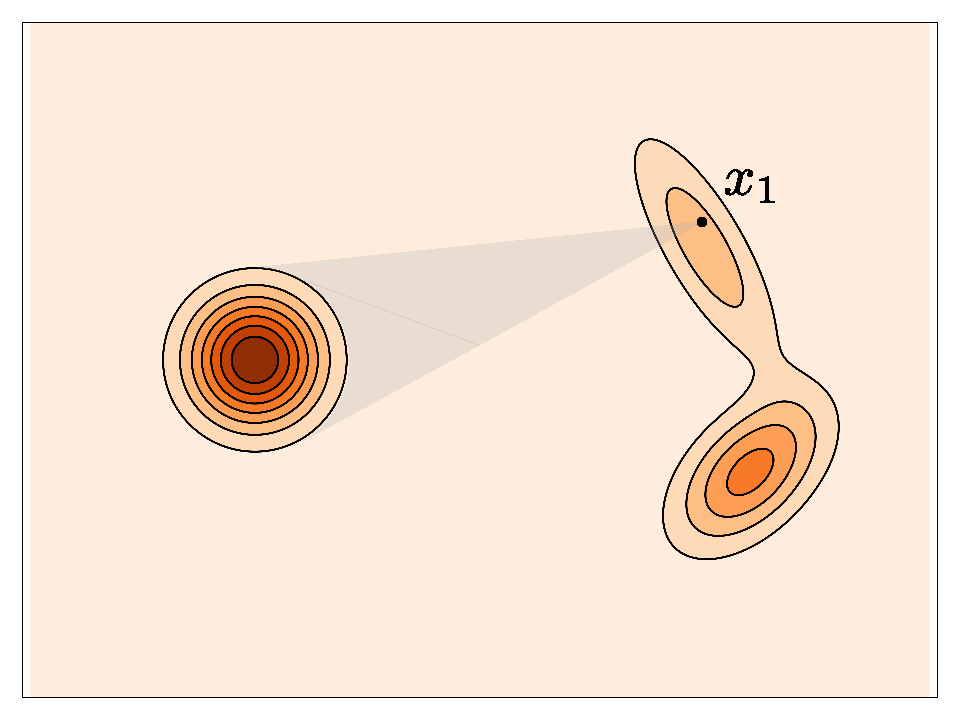
\includegraphics[width=0.9\textwidth]{assets/x1_cond.pdf}
        \end{figure}
        \begin{figure}
          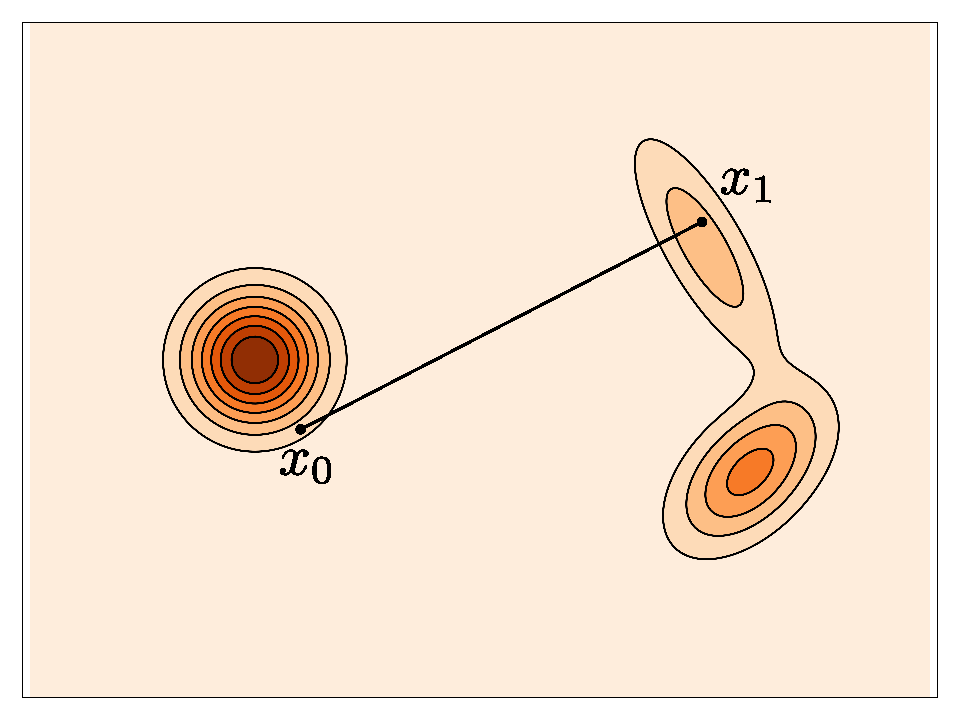
\includegraphics[width=0.9\textwidth]{assets/x0_x1_cond.pdf}
        \end{figure}
      \end{column}
      \begin{column}{0.65\textwidth}
        \begin{itemize}
          \item Optimal Transport (OT) is finding a optimal probability path $p_t^\star$ and velocity field $u_t^\star$ that safisfying
          $$
            (p^\star_t, u^\star_t) = \arg \min_{p_t, u_t} \int^1_0 \mbb{E}_{X_t \sim p_t} \lVert u_t(X_t)\rVert^2 dt
          $$
          \item Since it is hard to solve the OT problem, we instead minimize the upper bound:
          $$
            \begin{aligned}
              \int^1_0 \mbb{E}_{X_t \sim p_t} \lVert u_t(X_t) \rVert^2 dt &= \int^1_0 \mbb{E}_{X_t \sim p_t} \left\lVert \mbb{E}\left[\frac{d}{dt} \psi_t (X_0|X_1)|X_t\right]\right\rVert^2 dt \\
              &\leq \int^1_0 \mbb{E}_{X_t \sim p_t} \mbb{E} \left[\left\lVert\frac{d}{dt} \psi_t (X_0|X_1)\right\rVert^2 \mid X_t \right]dt \\ &= \mbb{E}_{X_0, X_1 \sim \pi_{0,1}} \int^1_0 \left\lVert \frac{d}{dt}\psi_t (X_0|X_1) \right\rVert^2 dt
            \end{aligned}
          $$
          \item This problem can be solved using Euler-Lagrange equations, which in this case take the form $\frac{d^2}{dt^2} \frac{d}{dt} \psi_t(x|x_1) = 0$, concluding
          $$
            \psi_t(x|x_1) = t x_1 + (1-t)x \implies u_t(x|x_1) = x_1 - x
          $$
          \item So flow matching loss is obtained by 
          $$
            \mc{L}_{\text{CFM}}(\theta) = \mbb{E}_{\substack{t \sim \Unif[0,1] \\ X_0, X_1 \sim \pi_{0,1}}} \left[ \left\lVert u_t(X_t|X_1)- u_t^\theta(X_t|X_1) \right\rVert^2 \right]
          $$
        \end{itemize}
      \end{column}
    \end{columns}
  \end{block}
\end{frame}

\begin{frame}{Appendix}
  \begin{block}{$C^r$ diffeomorphism} \label{appendix:diffeomorphism}
    We denote by $C^r(\mbb{R}^m, \mbb{R}^n)$ the collection of functions $f: \mbb{R}^m \to \mbb{R}^n$ with continuous derivatives of order $r$:
    $$
      \frac{\partial^r f^k}{\partial x^{i_1} \cdots \partial x^{i_r}}, \quad k \in \{1,2,\dots, n\}, i_j \in \{1, 2, \dots, m\}
    $$
    A map $f: \mbb{R}^n \to \mbb{R}^n$ is a $C^r$ \tb{diffeomorphism} if $f \in C^r(\mbb{R}^n, \mbb{R}^n)$ and its inverse $f^{-1}$ exists and satisfies $f^{-1} \in C^r(\mbb{R}^n, \mbb{R}^n)$.
  \end{block}
  \begin{block}{Flow Model is a Markov process} \label{appendix:flow_model_markov}
    $$
      X_s = \psi_s(X_0) = \psi_s (\psi^{-1}(\psi_t(X_0))) = \psi_{s|t}(X_t), \text{ where } \psi_{s|t} \triangleq \psi_s \circ \psi_t^{-1}
    $$
  \end{block}
\end{frame}

\begin{frame}{Appendix}
    \begin{block}{Continuity Equation and Mass Conservation} \label{appendix:continuity_equation_and_mass_conservation}
    To verify that a velocity field $u_t$ generates a probability path $p_t$, one can verify if the pair $(u_t, p_t)$ satisfies a partial differential equation (PDE) known as the \underline{Continuity Equation}:
    $$
      \frac{d}{dt}p_t(x) + \diverg(p_t u_t)(x) = 0
    $$
    where $\diverg(v)(x) = \sum^d_{i=1} \partial_{x^i} v^i(x)$, and $v(x) = (v^1(x), \dots, v^d(x))$.

    The following theorem, a rephrased version of the \underline{Math Conservation Formula}, states that a solution $u_t$ to the Continuity Equation generates the probability path $p_t$

    \begin{theorem}[Mass Conservation]
      Let $p_t$ be a probability path and $u_t$ a locally Lipchitz integrable vector field. Then, the following two statements are equivalent:
      \begin{enumerate}
        \item The Continuity Equation holds for $t \in [0,1)$
        \item $u_t$ generates $p_t$
      \end{enumerate}
    \end{theorem}
  \end{block}
\end{frame}

\begin{frame}{Appendix}
  \begin{block}{Bregman Divergence}\label{appendix:bregman_divergence}
    \begin{columns}
      \begin{column}{0.3\textwidth}
        \begin{figure}
          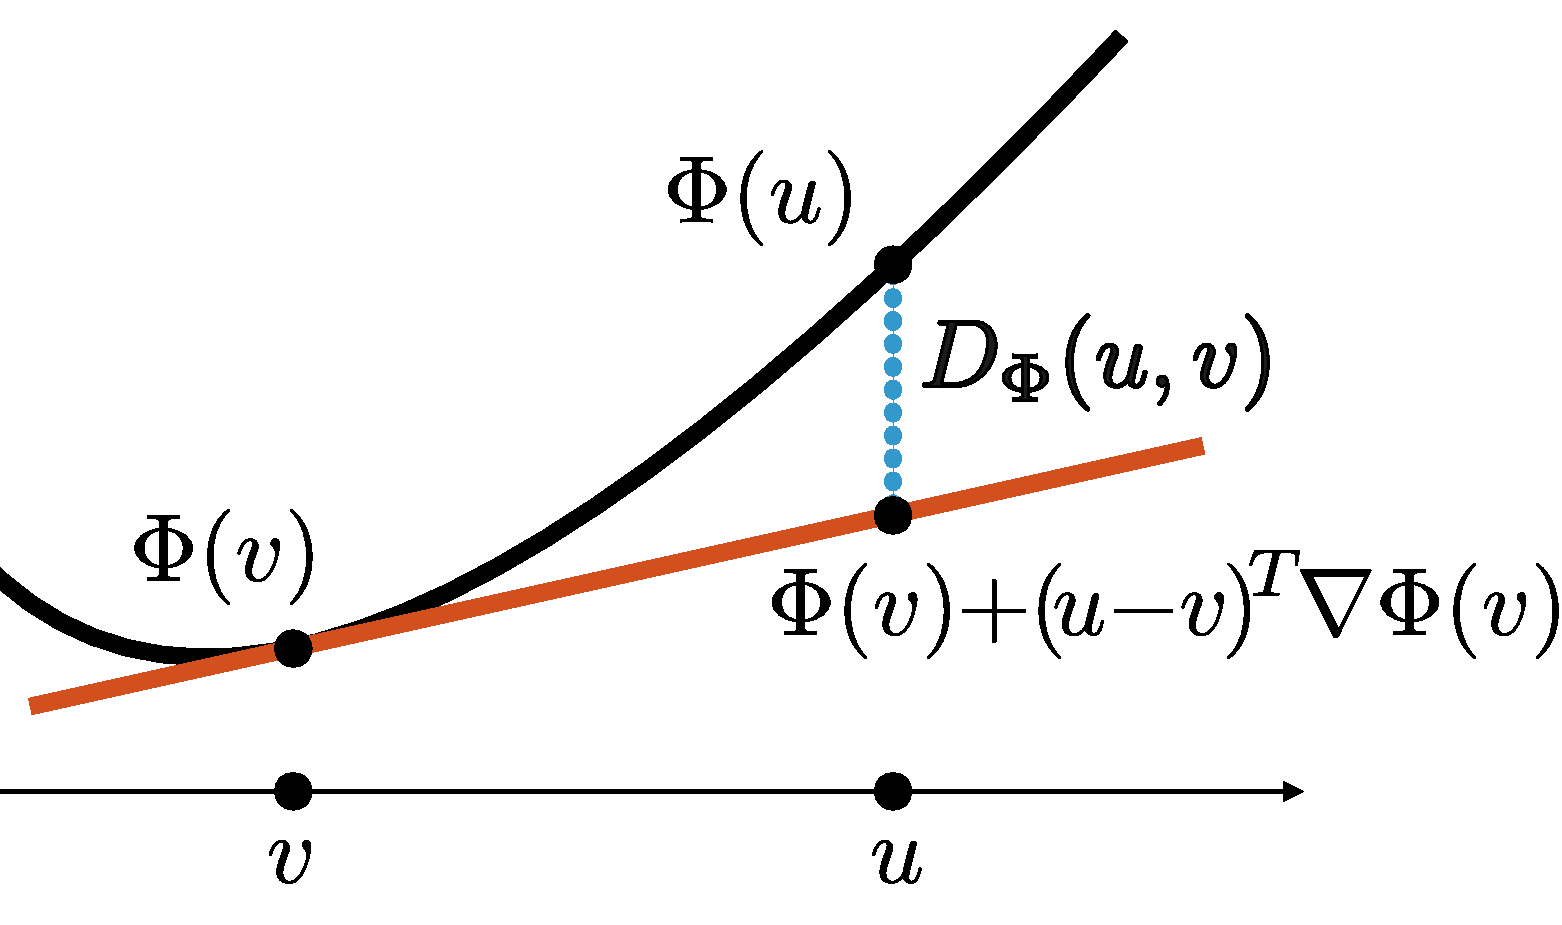
\includegraphics[width=0.9\textwidth]{assets/bregman.pdf}
        \end{figure}
      \end{column}
      \begin{column}{0.65\textwidth}
        For any vectors $u, v \in \mbb{R}^d$,
        $$
          D(u,v) \triangleq \Phi(u) -[\Phi(v) + \langle u - v, \nabla \Phi(v) \rangle]
        $$
        where $\phi: \mbb{R}^d \to \mbb{R}$ is a strictly convex function defined over some convex set $\Omega \subset \mbb{R}^d$.
      \end{column}
    \end{columns}
  \end{block}
\end{frame}

\end{document}